\chapter{Sistemas de ecuaciones\\Álgebra  II -- Año 2024/1 -- FAMAF}\label{practico-2}

\centerline{\textsc{}}

\subsection*{Objetivos}

\begin{itemize}
 \item Aprender a plantear y resolver sistemas de ecuaciones lineales.
\end{itemize}

\begin{enumerate}[topsep=6pt, itemsep=.4cm]
\item {\it Juego Suko}. Colocar los números del $1$ al $9$ en las celdas de la siguiente tabla de modo que el número en cada círculo sea igual a la suma de las cuatro celdas adyacentes, y la suma de las celdas del mismo color sea igual al número en el círculo de igual color.

\begin{center}
  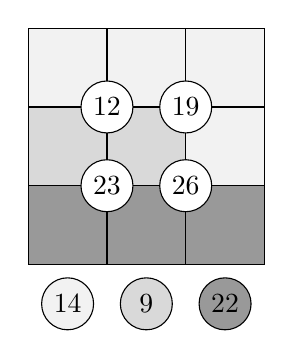
\begin{tikzpicture}
    \draw [fill=gray!10] (0,0) rectangle (1,-1); 
    \draw [fill=gray!10] (1,0) rectangle (2,-1); 
    \draw [fill=gray!10] (2,0) rectangle (3,-1); 
    \draw [fill=gray!30] (0,-1) rectangle (1,-2); 
    \draw [fill=gray!30] (1,-1) rectangle (2,-2); 
    \draw [fill=gray!10] (2,-1) rectangle (3,-2); 
    \draw [fill=gray!80] (0,-2) rectangle (1,-3); 
    \draw [fill=gray!80] (1,-2) rectangle (2,-3); 
    \draw [fill=gray!80] (2,-2) rectangle (3,-3); 
    \filldraw[fill=white](1,-1) circle (0.33);
    \filldraw[fill=white](2,-1) circle (0.33);
    \filldraw[fill=white](1,-2) circle (0.33);
    \filldraw[fill=white](2,-2) circle (0.33);
    \node at (1,-1) {12};
    \node at (2,-1) {19};
    \node at (1,-2) {23};
    \node at (2,-2) {26};
    \filldraw[fill=gray!10](0.5,-3.5) circle (0.33);
    \filldraw[fill=gray!30](1.5,-3.5) circle (0.33);
    \filldraw[fill=gray!80](2.5,-3.5) circle (0.33);
    \node at (0.5,-3.5) {14};
    \node at (1.5,-3.5) {9};
    \node at (2.5,-3.5) {22};
    
    \end{tikzpicture}
\end{center}



\item\label{polinomio} Encontrar los coeficientes reales del polinomio $p(x) = ax^2+bx+c$ de manera tal que $p(1)=2$, $p(2)=7$ y $p(3)=14$.



\item Determinar cuáles de las siguientes matrices son MERF.
$$\begin{array}{lccccl}
\begin{bmatrix}1 & 2 & 0 \\0 & 0 & 1 \end{bmatrix}, &
\begin{bmatrix}1 & 0 & 2 \\0 & 1 & -3 \end{bmatrix}, &
\begin{bmatrix}0 & 1 & 0 \\0 & 0 & 1 \end{bmatrix}, &
\begin{bmatrix}0 & 1 & 0 \\0 & 0 & 0 \end{bmatrix}, &
\begin{bmatrix}1 & 0 & 0  \\0 & 0 & 1 \\0 & 0 & 1 \end{bmatrix},&
\begin{bmatrix}1 & 0 & 0  \\0 & 0 & 0 \\0 & 0 & 1 \end{bmatrix}.
\end{array}$$



\item Para cada una de las MERF del ejercicio anterior,

\begin{enumerate}
\item
asumir que es la matriz de un sistema homogéneo, escribir el sistema
y dar las soluciones del sistema.

\item
asumir que es la matriz ampliada de un sistema no homogéneo, escribir el sistema
y dar las soluciones del sistema.
\end{enumerate}



\item\label{sistemas homogeneos} Para cada uno de los siguientes sistemas de ecuaciones, describir explícita o paramétricamente todas las soluciones e indicar cuál es la MERF asociada al sistema.

\begin{multicols}{2}
\begin{enumerate}
\item $\begin{cases}
 -x - y + 4z = 0\\
 x+3y+8z = 0\\
 x+2y + 5z = 0
\end{cases}$
\item $\begin{cases}
 x - 3y + 5z = 0\\
 2x-3y+z = 0\\
 -y + 3z = 0
\end{cases}$

\item $\begin{cases}
x-z+2t = 0\\
-x+2y-z+2t = 0\\
-x+y = 0
\end{cases}$

\item[(d)] $\begin{cases}
 -x - y + 4z = 1\\
 x+3y+8z = 3\\
 x+2y + 5z = 1
\end{cases}$

\item[(e)] $\begin{cases}
 x - 3y + 5z = 1\\
 2x-3y+z = 3\\
 -y + 3z = 1
\end{cases}$


\item[(f)] $\begin{cases}
x-z+2t = 1\\
-x+2y-z+2t = 3\\
-x+y = 1
\end{cases}$

\end{enumerate}
\end{multicols}



\item\label{sistemas con soluciones} Para cada uno de los siguientes sistemas, describir implícitamente el conjunto de los vectores $(b_1,b_2,b_3)$
o $(b_1,b_2,b_3,b_4)$ para los cuales cada sistema tiene solución.
\begin{multicols}{2}
\begin{enumerate}

\item $\begin{cases}
 x - 3y + 5z = b_1\\
 2x-3y+z = b_2\\
 -y + 3z = b_3
\end{cases}$


\item
$\begin{cases}
x-z+2t = b_1\\
-x+2y-z+2t = b_2\\
-x+y = b_3\\
y-z+2t=b_4
\end{cases}$


\item  \vskip .4cm  $\begin{cases}
 - x - y + 4 z = b_1\\
 x+3y+8z = b_2\\
 x + 2y + 5z = b_3
\end{cases}$

\end{enumerate}
\end{multicols}



\item Sea $A=\begin{bmatrix}1 & 2 & 3 & \cdots & 2016 \\ 2 & 3 & 4 & \cdots & 2017 \\ 3&4&5& \cdots & 2018\\ \vdots & &&& \vdots \\ 100 & 101 & 102& \cdots& 2115\end{bmatrix}$.


\begin{enumerate}
   \item Encontrar todas las soluciones del sistema $AX=0$.
   \item Encontrar todas las soluciones del sistema $AX=\left[\begin{array}{c}
     1\\\vdots \\1 \end{array}\right]$.
\end{enumerate}



     \item Sea $A=\begin{bmatrix}3 & -1 & 2 \\2 & 1 & 1 \\1&-3&0\end{bmatrix}$. Reduciendo $A$ por filas,
 \begin{enumerate}
   \item encontrar todas las soluciones sobre $\mathbb{R}$ y $\mathbb{C}$ del sistema $AX=0$.
   \item encontrar todas las soluciones sobre $\mathbb{R}$ y $\mathbb{C}$ del sistema $AX=\left[\begin{array}{c}
     1\\i\\0 \end{array}\right]$.
 \end{enumerate}


\item Suponga que tiene que resolver un sistema de ecuaciones lineales homogéneo y que tras hacer algunas operaciones elementales por fila a la matriz asociada obtiene una matriz con la siguiente forma
\begin{align*}
\left(
\begin{array}{cccc}
a & * & * & *\\
0 & b & * & *\\
0 & 0 & c & *\\
0 & 0 & 0 & d
\end{array}
\right)
\end{align*}
donde $a,b,c,d\in\R$ y $*$ son algunos números reales.
¿Qué conclusiones puede inferir acerca del conjunto de soluciones a partir de los valores de $a$, $b$, $c$ y $d$?



\item Suponga que tiene que resolver un sistema de ecuaciones lineales y que tras hacer algunas operaciones elementales por fila a la matriz ampliada obtiene una matriz con la siguiente forma
\begin{align*}
\left(
\begin{array}{cccc|c}
a & * & * & * & *\\
0 & b & * & * & *\\
0 & 0 & 0 & 0 & c\\
0 & 0 & 0 & d & *
\end{array}
\right)
\end{align*}
donde $a,b,c,d\in\R$ y $*$ son algunos números reales.
¿Qué conclusiones puede inferir acerca del conjunto de soluciones a partir de los valores de $a$, $b$, $c$ y $d$?



\item\label{soluciones-ecuaciones} Suponga que tiene que resolver un sistema de $m$ ecuaciones lineales con $n$ incógnitas. Antes de empezar a hacer cuentas y apelando a la teoría, ¿Qué puede afirmar acerca del conjunto de soluciones en base a $m$ y $n$? ¿Cómo saber si es vacío o no vacío? ¿Si tiene una o varias soluciones?




\item\label{polinomios} $\textcircled{a}$ Sean $\lambda_1, ..., \lambda_n\in\R$ y $b_1, ..., b_n\in\R$.


\begin{enumerate}
 \item\label{polinomios-a} Para cada $n\in\{1,2,3,4,5\}$, plantear un sistema de ecuaciones lineales que le permita encontrar un polinomio $p(x)$ con coeficientes reales de grado $n-1$ tal que
 $$
 p(\lambda_1)=b_1, \dots, p(\lambda_n)=b_n.
 $$
\item\label{polinomios-b} ¿Se le ocurre alguna condición con la cual pueda afirmar que el sistema anterior no tiene solución?
\item\label{polinomios-c}  ¿Puede dar una forma general del sistema para cualquier $n$?
\end{enumerate}


\end{enumerate}














